\documentclass[border=10pt, tikz]{standalone}
\usetikzlibrary{arrows.meta}

\definecolor{curveblue}{HTML}{B2D7EA} % Filling
\definecolor{jumpred}{HTML}{E97AB1}   % Vertical jump line
\definecolor{textdark}{HTML}{222222}

\begin{document}
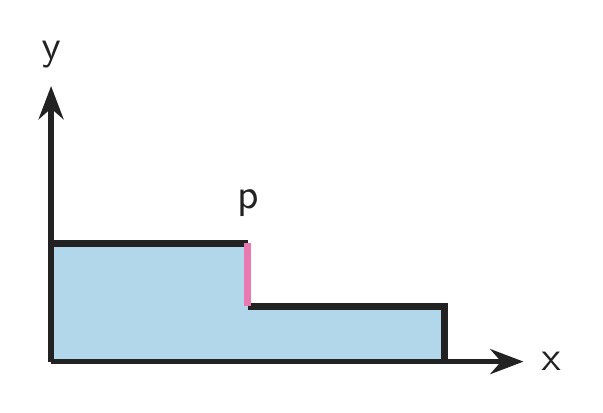
\begin{tikzpicture}[font=\sffamily, >=Stealth]

    % Area Filling
    \fill[curveblue] (0,0) -- (0,1.5) -- (2.5, 1.5) -- (2.5, 0.7) -- (5, 0.7) -- (5,0) -- cycle;
    
    % Axes
    \draw[line width=2pt, ->, textdark] (0,0) -- (6,0) node[right, scale=1.5] {x};
    \draw[line width=2pt, ->, textdark] (0,0) -- (0,3.5) node[above, scale=1.5] {y};
    
    % Step Function Outline
    \draw[line width=2.5pt, textdark] (0,1.5) -- (2.5,1.5);
    \draw[line width=2.5pt, textdark] (2.5, 0.7) -- (5, 0.7) -- (5,0);
    
    % Highlighted Jump at p
    \draw[jumpred, line width=2.5pt] (2.5, 0.7) -- (2.5, 1.5) 
        node[above, textdark, scale=1.5, yshift=2pt] {p};

\end{tikzpicture}
\end{document}